
%-----------------------------------------------------------------------------
% PACKAGES AND OTHER DOCUMENT CONFIGURATIONS
%-----------------------------------------------------------------------------

\documentclass[11pt]{article}
% \usepackage[margin=1in]{geometry}
% \usepackage{amsmath, amsfonts}
% \usepackage{enumerate}
% \usepackage{graphicx}
% \usepackage{titling}
% \usepackage{url}
% \usepackage{xfrac}
% \usepackage{fancyhdr}
% \usepackage{geometry}
% \usepackage{graphicx}
% \usepackage{natbib}
% \usepackage{amsmath}
% \usepackage{amssymb}
% \usepackage{amsthm}
% \usepackage{paralist}
% \usepackage{epstopdf}
% \usepackage{tabularx}
% \usepackage{longtable}
% \usepackage{multirow}
% \usepackage{multicol}
% \usepackage[colorlinks=true,urlcolor=blue]{hyperref}
% \usepackage{fancyvrb}
% \usepackage{algorithm}
% \usepackage{algorithmicx}
% \usepackage[noend]{algpseudocode}
% \usepackage{float}
% \usepackage{paralist}
% \usepackage[svgname]{xcolor}
% \usepackage{enumerate}
% \usepackage{array}
% \usepackage{times}
% \usepackage{url}
% \usepackage{fancyhdr}
% \usepackage{comment}
% \usepackage{environ}
% \usepackage{times}
% \usepackage{textcomp}
% \usepackage{caption}
% \usepackage[colorlinks=true,urlcolor=blue]{hyperref}
% \usepackage{parskip} % For NIPS style paragraphs.
% \usepackage[compact]{titlesec} % Less whitespace around titles
% \usepackage[inline]{enumitem} % For inline enumerate* and itemize*
% \usepackage{datetime}
% \usepackage{comment}
% %\usepackage{minted}
% \usepackage{lastpage}
% \usepackage{color}
% \usepackage{xcolor}
% \usepackage[final]{listings}
% \usepackage{tikz}
% \usetikzlibrary{positioning, arrows, automata}
% \usetikzlibrary{shapes,decorations}
% \usepackage{framed}
% \usepackage{booktabs}
% \usepackage{cprotect}
% \usepackage{fancyvrb}
% \usepackage{xcolor}
% \usepackage{verbatimbox}
% \usepackage{multicol}
% \usepackage{hyperref}
% \usepackage{subcaption}
% \usepackage{mathtools} % For drcases
% \usepackage[many]{tcolorbox}

\usepackage{amsmath, amssymb, amsthm, enumerate, graphicx}
\usepackage[usenames,dvipsnames]{color}
\usepackage{bm}
\usepackage[colorlinks=true,urlcolor=blue]{hyperref}
\usepackage{geometry}
\geometry{margin=1in}
\usepackage{float}
\usepackage{graphics}
\setlength{\marginparwidth}{2.15cm}
\usepackage{booktabs}
\usepackage{enumitem}
\usepackage{epsfig}
\usepackage{setspace}
\usepackage{parskip}
\usepackage[normalem]{ulem}
\usepackage{tikz}
\usetikzlibrary{positioning, arrows, automata}
\usepackage{pgfplots}
\pgfplotsset{compat=newest}
\usepackage[font=scriptsize]{subcaption}
\usepackage{float}
\usepackage[]{algorithm2e}
\usepackage{environ}
\usepackage{bbm}
\usepackage{graphicx}
\usepackage{titling}
\usepackage{url}
\usepackage{xcolor}
\usepackage{lipsum}
\usepackage{lastpage}
\usepackage[colorlinks=true,urlcolor=blue]{hyperref}
\usepackage{multicol}
\usepackage{tabularx}
\usepackage{comment}
\usepackage[utf8]{inputenc}
\usepackage{amssymb}
\usepackage{setspace}
\usepackage{marvosym}
\usepackage{wrapfig}
\usepackage{datetime}
\usepackage[many]{tcolorbox}
\usepackage{array}
\usepackage{multirow}
\usepackage{wasysym}
\usepackage{cancel}
\usepackage{cprotect}
\usepackage{listings}
\usepackage{color}


%%%%%%%%%%%%%%%%%%%%%%%%%%%%%%%%%%%%%%%%%%%
% Better numbering                        %
%%%%%%%%%%%%%%%%%%%%%%%%%%%%%%%%%%%%%%%%%%%

\numberwithin{equation}{section} % Number equations within sections (i.e. 1.1, 1.2, 2.1, 2.2 instead of 1, 2, 3, 4)
\numberwithin{figure}{section} % Number figures within sections (i.e. 1.1, 1.2, 2.1, 2.2 instead of 1, 2, 3, 4)
\numberwithin{table}{section} % Number tables within sections (i.e. 1.1, 1.2, 2.1, 2.2 instead of 1, 2, 3, 4)

%%%%%%%%%%%%%%%%%%%%%%%%%%%%%%%%%%%%%%%%%%
% Custom commands                        %
%%%%%%%%%%%%%%%%%%%%%%%%%%%%%%%%%%%%%%%%%%

\newcommand{\vc}[1]{\boldsymbol{#1}}
\newcommand{\adj}[1]{\frac{d J}{d #1}}
\newcommand{\chain}[2]{\adj{#2} = \adj{#1}\frac{d #1}{d #2}}

\newcommand{\R}{\mathbb{R}}
\newcommand{\blackcircle}{\tikz\draw[black,fill=black] (0,0) circle (1ex);}
\renewcommand{\circle}{\tikz\draw[black] (0,0) circle (1ex);}


% mathcal
\newcommand{\Ac}{\mathcal{A}}
\newcommand{\Bc}{\mathcal{B}}
\newcommand{\Cc}{\mathcal{C}}
\newcommand{\Dc}{\mathcal{D}}
\newcommand{\Ec}{\mathcal{E}}
\newcommand{\Fc}{\mathcal{F}}
\newcommand{\Gc}{\mathcal{G}}
\newcommand{\Hc}{\mathcal{H}}
\newcommand{\Ic}{\mathcal{I}}
\newcommand{\Jc}{\mathcal{J}}
\newcommand{\Kc}{\mathcal{K}}
\newcommand{\Lc}{\mathcal{L}}
\newcommand{\Mc}{\mathcal{M}}
\newcommand{\Nc}{\mathcal{N}}
\newcommand{\Oc}{\mathcal{O}}
\newcommand{\Pc}{\mathcal{P}}
\newcommand{\Qc}{\mathcal{Q}}
\newcommand{\Rc}{\mathcal{R}}
\newcommand{\Sc}{\mathcal{S}}
\newcommand{\Tc}{\mathcal{T}}
\newcommand{\Uc}{\mathcal{U}}
\newcommand{\Vc}{\mathcal{V}}
\newcommand{\Wc}{\mathcal{W}}
\newcommand{\Xc}{\mathcal{X}}
\newcommand{\Yc}{\mathcal{Y}}
\newcommand{\Zc}{\mathcal{Z}}

% mathbb
\newcommand{\Ab}{\mathbb{A}}
\newcommand{\Bb}{\mathbb{B}}
\newcommand{\Cb}{\mathbb{C}}
\newcommand{\Db}{\mathbb{D}}
\newcommand{\Eb}{\mathbb{E}}
\newcommand{\Fb}{\mathbb{F}}
\newcommand{\Gb}{\mathbb{G}}
\newcommand{\Hb}{\mathbb{H}}
\newcommand{\Ib}{\mathbb{I}}
\newcommand{\Jb}{\mathbb{J}}
\newcommand{\Kb}{\mathbb{K}}
\newcommand{\Lb}{\mathbb{L}}
\newcommand{\Mb}{\mathbb{M}}
\newcommand{\Nb}{\mathbb{N}}
\newcommand{\Ob}{\mathbb{O}}
\newcommand{\Pb}{\mathbb{P}}
\newcommand{\Qb}{\mathbb{Q}}
\newcommand{\Rb}{\mathbb{R}}
\newcommand{\Sb}{\mathbb{S}}
\newcommand{\Tb}{\mathbb{T}}
\newcommand{\Ub}{\mathbb{U}}
\newcommand{\Vb}{\mathbb{V}}
\newcommand{\Wb}{\mathbb{W}}
\newcommand{\Xb}{\mathbb{X}}
\newcommand{\Yb}{\mathbb{Y}}
\newcommand{\Zb}{\mathbb{Z}}

% mathbf lowercase
\newcommand{\av}{\mathbf{a}}
\newcommand{\bv}{\mathbf{b}}
\newcommand{\cv}{\mathbf{c}}
\newcommand{\dv}{\mathbf{d}}
\newcommand{\ev}{\mathbf{e}}
\newcommand{\fv}{\mathbf{f}}
\newcommand{\gv}{\mathbf{g}}
\newcommand{\hv}{\mathbf{h}}
\newcommand{\iv}{\mathbf{i}}
\newcommand{\jv}{\mathbf{j}}
\newcommand{\kv}{\mathbf{k}}
\newcommand{\lv}{\mathbf{l}}
\newcommand{\mv}{\mathbf{m}}
\newcommand{\nv}{\mathbf{n}}
\newcommand{\ov}{\mathbf{o}}
\newcommand{\pv}{\mathbf{p}}
\newcommand{\qv}{\mathbf{q}}
\newcommand{\rv}{\mathbf{r}}
\newcommand{\sv}{\mathbf{s}}
\newcommand{\tv}{\mathbf{t}}
\newcommand{\uv}{\mathbf{u}}
\newcommand{\vv}{\mathbf{v}}
\newcommand{\wv}{\mathbf{w}}
\newcommand{\xv}{\mathbf{x}}
\newcommand{\yv}{\mathbf{y}}
\newcommand{\zv}{\mathbf{z}}

% mathbf uppercase
\newcommand{\Av}{\mathbf{A}}
\newcommand{\Bv}{\mathbf{B}}
\newcommand{\Cv}{\mathbf{C}}
\newcommand{\Dv}{\mathbf{D}}
\newcommand{\Ev}{\mathbf{E}}
\newcommand{\Fv}{\mathbf{F}}
\newcommand{\Gv}{\mathbf{G}}
\newcommand{\Hv}{\mathbf{H}}
\newcommand{\Iv}{\mathbf{I}}
\newcommand{\Jv}{\mathbf{J}}
\newcommand{\Kv}{\mathbf{K}}
\newcommand{\Lv}{\mathbf{L}}
\newcommand{\Mv}{\mathbf{M}}
\newcommand{\Nv}{\mathbf{N}}
\newcommand{\Ov}{\mathbf{O}}
\newcommand{\Pv}{\mathbf{P}}
\newcommand{\Qv}{\mathbf{Q}}
\newcommand{\Rv}{\mathbf{R}}
\newcommand{\Sv}{\mathbf{S}}
\newcommand{\Tv}{\mathbf{T}}
\newcommand{\Uv}{\mathbf{U}}
\newcommand{\Vv}{\mathbf{V}}
\newcommand{\Wv}{\mathbf{W}}
\newcommand{\Xv}{\mathbf{X}}
\newcommand{\Yv}{\mathbf{Y}}
\newcommand{\Zv}{\mathbf{Z}}

% bold greek lowercase
\newcommand{\alphav     }{\boldsymbol \alpha     }
\newcommand{\betav      }{\boldsymbol \beta      }
\newcommand{\gammav     }{\boldsymbol \gamma     }
\newcommand{\deltav     }{\boldsymbol \delta     }
\newcommand{\epsilonv   }{\boldsymbol \epsilon   }
\newcommand{\varepsilonv}{\boldsymbol \varepsilon}
\newcommand{\zetav      }{\boldsymbol \zeta      }
\newcommand{\etav       }{\boldsymbol \eta       }
\newcommand{\thetav     }{\boldsymbol \theta     }
\newcommand{\varthetav  }{\boldsymbol \vartheta  }
\newcommand{\iotav      }{\boldsymbol \iota      }
\newcommand{\kappav     }{\boldsymbol \kappa     }
\newcommand{\varkappav  }{\boldsymbol \varkappa  }
\newcommand{\lambdav    }{\boldsymbol \lambda    }
\newcommand{\muv        }{\boldsymbol \mu        }
\newcommand{\nuv        }{\boldsymbol \nu        }
\newcommand{\xiv        }{\boldsymbol \xi        }
\newcommand{\omicronv   }{\boldsymbol \omicron   }
\newcommand{\piv        }{\boldsymbol \pi        }
\newcommand{\varpiv     }{\boldsymbol \varpi     }
\newcommand{\rhov       }{\boldsymbol \rho       }
\newcommand{\varrhov    }{\boldsymbol \varrho    }
\newcommand{\sigmav     }{\boldsymbol \sigma     }
\newcommand{\varsigmav  }{\boldsymbol \varsigma  }
\newcommand{\tauv       }{\boldsymbol \tau       }
\newcommand{\upsilonv   }{\boldsymbol \upsilon   }
\newcommand{\phiv       }{\boldsymbol \phi       }
\newcommand{\varphiv    }{\boldsymbol \varphi    }
\newcommand{\chiv       }{\boldsymbol \chi       }
\newcommand{\psiv       }{\boldsymbol \psi       }
\newcommand{\omegav     }{\boldsymbol \omega     }

% bold greek uppercase
\newcommand{\Gammav     }{\boldsymbol \Gamma     }
\newcommand{\Deltav     }{\boldsymbol \Delta     }
\newcommand{\Thetav     }{\boldsymbol \Theta     }
\newcommand{\Lambdav    }{\boldsymbol \Lambda    }
\newcommand{\Xiv        }{\boldsymbol \Xi        }
\newcommand{\Piv        }{\boldsymbol \Pi        }
\newcommand{\Sigmav     }{\boldsymbol \Sigma     }
\newcommand{\Upsilonv   }{\boldsymbol \Upsilon   }
\newcommand{\Phiv       }{\boldsymbol \Phi       }
\newcommand{\Psiv       }{\boldsymbol \Psi       }
\newcommand{\Omegav     }{\boldsymbol \Omega     }

%%%%%%%%%%%%%%%%%%%%%%%%%%%%%%%%%%%%%%%%%%%
% Code highlighting with listings         %
%%%%%%%%%%%%%%%%%%%%%%%%%%%%%%%%%%%%%%%%%%%

\definecolor{bluekeywords}{rgb}{0.13,0.13,1}
\definecolor{greencomments}{rgb}{0,0.5,0}
\definecolor{redstrings}{rgb}{0.9,0,0}
\definecolor{light-gray}{gray}{0.95}

\newcommand{\MYhref}[3][blue]{\href{#2}{\color{#1}{#3}}}%

\definecolor{dkgreen}{rgb}{0,0.6,0}
\definecolor{gray}{rgb}{0.5,0.5,0.5}
\definecolor{mauve}{rgb}{0.58,0,0.82}

\lstdefinelanguage{Shell}{
  keywords={tar, cd, make},
  %keywordstyle=\color{bluekeywords}\bfseries,
  alsoletter={+},
  ndkeywords={python, py, javac, java, gcc, c, g++, cpp, .txt, octave, m, .tar},
  %ndkeywordstyle=\color{bluekeywords}\bfseries,
  identifierstyle=\color{black},
  sensitive=false,
  comment=[l]{//},
  morecomment=[s]{/*}{*/},
  commentstyle=\color{purple}\ttfamily,
  %stringstyle=\color{red}\ttfamily,
  morestring=[b]',
  morestring=[b]",
  backgroundcolor = \color{light-gray}
}

\lstset{columns=fixed, basicstyle=\ttfamily,
    backgroundcolor=\color{light-gray},xleftmargin=0.5cm,frame=tlbr,framesep=4pt,framerule=0pt}


%%%%%%%%%%%%%%%%%%%%%%%%%%%%%%%%%%%%%%%%%%%
% Custom box for highlights               %
%%%%%%%%%%%%%%%%%%%%%%%%%%%%%%%%%%%%%%%%%%%

% Define box and box title style
\tikzstyle{mybox} = [fill=blue!10, very thick,
    rectangle, rounded corners, inner sep=1em, inner ysep=1em, text width=\dimexpr\linewidth-22pt]

% \newcommand{\notebox}[1]{
% \begin{tikzpicture}
% \node [mybox] (box){%
%     \begin{minipage}{\textwidth}
%     #1
%     \end{minipage}
% };
% \end{tikzpicture}%
% }

\NewEnviron{notebox}{

\begin{tikzpicture}
\node [mybox] (box){
    \begin{minipage}{\textwidth}
        \BODY
    \end{minipage}
};
\end{tikzpicture}
}

%%%%%%%%%%%%%%%%%%%%%%%%%%%%%%%%%%%%%%%%%%%%%%%%%
% Useful commands for typesetting the questions %
%%%%%%%%%%%%%%%%%%%%%%%%%%%%%%%%%%%%%%%%%%%%%%%%%

\newcommand{\points}[1]{{\bf [#1 points]}}
\newcommand \expect {\mathbb{E}}
\newcommand \mle [1]{{\hat #1}^{\rm MLE}}
\newcommand \map [1]{{\hat #1}^{\rm MAP}}
\newcommand \argmax {\operatorname*{argmax}}
\newcommand \argmin {\operatorname*{argmin}}
\newcommand \code [1]{{\tt #1}}
\newcommand \datacount [1]{\#\{#1\}}
\newcommand \ind [1]{\mathbb{I}\{#1\}}

%%%%%%%%%%%%%%%%%%%%%%%%%%
% Document configuration %
%%%%%%%%%%%%%%%%%%%%%%%%%%

% Don't display a date in the title and remove the white space
\predate{}
\postdate{}
\date{}

% Don't display an author and remove the white space
%\preauthor{}
%\postauthor{}

%%%%%%%%%%%%%%%%%%
% Begin Document %
%%%%%%%%%%%%%%%%%% 

\begin{document}


\section*{}
\begin{center}
  \centerline{\textsc{\LARGE  Homework 6}}
  \vspace{0.5em}
  \centerline{\textsc{\LARGE Information Theory and Reinforcement Learning}\footnote{Compiled on \today{} at \currenttime{}}}
  \vspace{1em}
  \textsc{\large CMU 10-601: Machine Learning (Fall 2019)} \\
  \vspace{0.5em}
  \url{https://piazza.com/class/jzcralyzwhu107} \\
  \vspace{0.5em}
  \centerline{OUT: Friday, Oct 25th, 2019}
  %\today{} at \currenttime{}}}
  \vspace{0.5em}
  \centerline{DUE: Friday, Nov 8th, 2019, 11:59pm}
    \centerline{TAs: Longxiang Zhang, David Xu, Yang Yu, Yuwei Qiu}
\end{center}

\section*{START HERE: Instructions}

\begin{notebox}
\paragraph{Summary} In this assignment, you will implement a reinforcement learning algorithm for solving the classic mountain-car environment. As a warmup, Section \ref{sec:warmup} will lead you through an on-paper example of how value iteration and Q-learning work. Then, in Section \ref{sec:code}, you will implement Q-learning with function approximation to solve the mountain car environment.
Apart from that, Section \ref{sec:warmup} will also cover questions of Information Theory to help you comprehend basic concepts.
\end{notebox}

\begin{itemize}

\item \textbf{Collaboration policy:} Collaboration on solving the homework is allowed, after you have thought about the problems on your own. It is also OK to get clarification (but not solutions) from books or online resources, again after you have thought about the problems on your own. There are two requirements: first, cite your collaborators fully and completely (e.g., ``Jane explained to me what is asked in Question 2.1''). Second, write your solution {\em independently}: close the book and all of your notes, and send collaborators out of the room, so that the solution comes from you only.  See the Academic Integrity Section on the course site for more information: \url{http://www.cs.cmu.edu/~mgormley/courses/10601/about.html#7-academic-integrity-policies}

\item\textbf{Late Submission Policy:} See the late submission policy here: \url{http://www.cs.cmu.edu/~mgormley/courses/10601/about.html#6-general-policies}

\item\textbf{Submitting your work:} You will use Gradescope to submit
  answers to all questions, and Autolab to submit your code. Please
  follow instructions at the end of this PDF to correctly submit all your code to Autolab.

  \begin{itemize}
    
  % COMMENT IF NOT USING CANVAS
\begin{comment}
  \item \textbf{Canvas:} Canvas (\url{https://canvas.cmu.edu}) will be
    used for quiz-style problems (e.g. multiple choice, true / false,
    numerical answers). Grading is done automatically.
    %
    You may only \textbf{submit once} on canvas, so be sure of your
    answers before you submit. However, canvas allows you to work on
    your answers and then close out of the page and it will save your
    progress.  You will not be granted additional submissions, so
    please be confident of your solutions when you are submitting your
    assignment.
    %
    {\color{red} The above is true for future assignments, but this one
    allows {\bf unlimited submissions}.}
\end{comment}
    
  % COMMENT IF NOT USING GRADESCOPE
   \item \textbf{Gradescope:} For written problems such as derivations,
       proofs, or plots we will be using Gradescope
       (\url{https://gradescope.com/}). Please use ther provided template. Submissions can be handwritten onto the template, but
       should be labeled and clearly legible. If your writing is not
       legible, you will not be awarded marks. Alternatively, submissions
       can be written in LaTeX. Regrade requests can be made, however
       this gives the TA the opportunity to regrade your entire paper,
       meaning if additional mistakes are found then points will be
       deducted.
       %   

  %   COMMENT IF NOT USING AUTOLAB
  \item \textbf{Autolab:} You will submit your code for programming
    questions on the homework to Autolab
    (\url{https://autolab.andrew.cmu.edu/}). After uploading your code,
    our grading scripts will autograde your assignment by running your
    program on a virtual machine (VM). 
    %
    When you are developing, check that the
    version number of the programming language environment
    (e.g. Python 2.7.6/3.6.8, Octave 3.8.2, OpenJDK 1.8.0, g++ 4.8.5) and
    versions of permitted libraries (e.g.  \texttt{numpy} 1.11.1 and \texttt{scipy} 0.18.1) 
    match those used on Autolab.
    % 
    (Octave users: Please make sure you do not use any
    Matlab-specific libraries in your code that might make it fail
    against our tests. Python3 users: Please pay special attention to the instructions at the end of this PDF)
    %
    You have a {\bf total of 10 Autolab submissions}. Use them
    %

  \end{itemize}
  
\item\textbf{Materials:} Download from Autolab the tar file (``Download
  handout"). The tar file will contain all the data that you will need in order to complete this assignment.

\end{itemize}

\clearpage
\section*{Instructions for Specific Problem Types}

For ``Select One" questions, please fill in the appropriate bubble completely:

\begin{quote}
\textbf{Select One:} Who taught this course?
\begin{list}{}
     \item\CIRCLE{} Matt Gormley
     \item\Circle{} Marie Curie
     \item\Circle{} Noam Chomsky
\end{list}
\end{quote}

If you need to change your answer, you may cross out the previous answer and bubble in the new answer:

\begin{quote}
\textbf{Select One:} Who taught this course?
\begin{list}{}
     \item\CIRCLE{} Matt Gormley
     \item\Circle{} Marie Curie\\
     \xcancel{\CIRCLE}{} Noam Chomsky
\end{list}
\end{quote}


For ``Select all that apply" questions, please fill in all appropriate squares completely:

\begin{quote}
\textbf{Select all that apply:} Which are scientists?
    \begin{list}{}
    \item $\blacksquare$ Stephen Hawking 
    \item $\blacksquare$ Albert Einstein
    \item $\blacksquare$ Isaac Newton
    \item $\square$ I don't know
\end{list}
\end{quote}

Again, if you need to change your answer, you may cross out the previous answer(s) and bubble in the new answer(s):

\begin{quote}
\textbf{Select all that apply:} Which are scientists?
    \begin{list}{}
    \item $\blacksquare$ Stephen Hawking 
    \item $\blacksquare$ Albert Einstein
    \item $\blacksquare$ Isaac Newton\\
    \xcancel{$\blacksquare$} I don't know
\end{list}
\end{quote}

For questions where you must fill in a blank, please make sure your final answer is fully included in the given space. You may cross out answers or parts of answers, but the final answer must still be within the given space.

\begin{quote}
\textbf{Fill in the blank:} What is the course number?

\begin{tcolorbox}[fit,height=1cm, width=4cm, blank, borderline={1pt}{-2pt},nobeforeafter]
    \begin{center}\huge10-601\end{center}
    \end{tcolorbox}\hspace{2cm}
    \begin{tcolorbox}[fit,height=1cm, width=4cm, blank, borderline={1pt}{-2pt},nobeforeafter]
    \begin{center}\huge10-\xcancel{7}601\end{center}
    \end{tcolorbox}
\end{quote}


\clearpage
\section{Written Questions \points{43+2}}
\label{sec:warmup}
Answer the following questions in the HW6 solutions template provided.  Then upload your solutions to Gradescope. You may use \LaTeX\ or print the template and hand-write your answers then scan it in. Failure to use the template may result in a penalty.
\subsection{Information Theory [15+2 points]}
\begin{enumerate}
    \item[1] [2 points] Given two fair six-sided dices. Let $S$ be the sum of the two faces of the dices after 1 roll. Answer the following questions:
    \begin{enumerate}
        \item How surprised are you, in bits, if $S=12$? Please round to three decimal places.\\
        \begin{tcolorbox}[fit,height=1cm, width=0.5\linewidth, blank, borderline={1pt}{-2pt},nobeforeafter]
        \begin{center}\huge5.170\end{center}
        \end{tcolorbox}
        \item What is the entropy of $S$? Please round to three decimal places.\\
        \begin{tcolorbox}[fit,height=1cm, width=0.5\linewidth, blank, borderline={1pt}{-2pt},nobeforeafter]
        \begin{center}\huge3.274\end{center}
        \end{tcolorbox}
    \end{enumerate}
    
    \item[2] [3 points] Following is a joint probability distribution table between two random variables $X$ and $Y$:\\
        \begin{tabular}{|l|l|l|l|}
        \hline
                  & $X=1$ & $X=0$ & $X=-1$ \\ \hline
        $Y=0$ & 0.15      & 0.225     & 0.0        \\ \hline
        $Y=1$ & 0.125     & 0.3       & 0.2        \\ \hline
        \end{tabular} \\
    Answer the following based on the table. Round all your answers to three decimal places:\\
    \begin{enumerate}
        \item What is $H(Y)$?
        \begin{tcolorbox}[fit,height=0.7cm, width=0.3\linewidth, blank, borderline={1pt}{-2pt}]
        \begin{center}\huge0.954\end{center}
        \end{tcolorbox}
        \item What is $H(Y|X)$?
        \begin{tcolorbox}[fit,height=0.7cm, width=0.3\linewidth, blank, borderline={1pt}{-2pt}]
        \begin{center}\huge0.445\end{center}
        \end{tcolorbox}
        \item What is the mutual information $I(Y;X)$?
        \begin{tcolorbox}[fit,height=0.7cm, width=0.3\linewidth, blank, borderline={1pt}{-2pt}]
        \begin{center}\huge0.509\end{center}
        \end{tcolorbox}
    \end{enumerate}
    
    \item[3] [5 points] Fill in the blank below with the \textbf{strongest} relational symbol ($<, >, \le, \ge, =, ?$) that is guaranteed to hold between the two sides. You can assume (i) all random variables are discrete (ii) all random variables have strictly positive entropy (iii) all capital letters represent random variables and all lowercase letters represent specific values. "?" is for no definite relationship. $H$ is the entropy, $CH$ the cross entropy and $I$ the mutual information\\
    \begin{enumerate}
        \item $H(X)$  \begin{tcolorbox}[fit,height=0.7cm, width=0.7cm, blank, borderline={1pt}{-2pt}, nobeforeafter]
        \begin{center}\huge$\ge$\end{center}
        \end{tcolorbox} $H(X|Y)$
        \item $H(X)$ \begin{tcolorbox}[fit,height=0.7cm, width=0.7cm, blank, borderline={1pt}{-2pt}, nobeforeafter]
        \begin{center}\huge$?$\end{center}
        \end{tcolorbox} $H(X|Y=y)$
        \item $CH(X, Y)$ \begin{tcolorbox}[fit,height=0.7cm, width=0.7cm, blank, borderline={1pt}{-2pt}, nobeforeafter]
        \begin{center}\huge$\ge$\end{center}
        \end{tcolorbox} $H(X)$
        \item $CH(X,Y)$ \begin{tcolorbox}[fit,height=0.7cm, width=0.7cm, blank, borderline={1pt}{-2pt}, nobeforeafter]
        \begin{center}\huge$?$\end{center}
        \end{tcolorbox} $H(X) + H(Y)$
        \item $I(X;Y|Z)$ \begin{tcolorbox}[fit,height=0.7cm, width=0.7cm, blank, borderline={1pt}{-2pt}, nobeforeafter]
        \begin{center}\huge$\ge$\end{center}
        \end{tcolorbox} $0$
    \end{enumerate}
    
    \item[4] [3 points] For two random variables $X$ and $Y$, draw a Venn diagram showing the relationship between the following quantities:
    \begin{enumerate}
        \item $H(X|Y)$
        \item $H(X, Y)$ 
        \item $I(X;Y)$ 
    \end{enumerate}
    \begin{tcolorbox}[fit,height=5cm, width=\linewidth, blank, borderline={1pt}{1pt}]
    \end{tcolorbox}
    
    
    \item[5] [2 points] Prove the symmetry of mutual information between any two random variables X,Y, i.e., $I(X;Y) = I(Y;X)$.\\
    \begin{tcolorbox}[fit,height=5cm, width=\linewidth, blank, borderline={1pt}{1pt}]
    \end{tcolorbox}
    
    
    \item[6] [bonus, 2 points] Can you come up with a joint probability distribution over three binary variables $X, Y, Z$ that satisfies the following properties?
    \begin{enumerate}
        \item $I(X;Z)=0$
        \item $I(Y;Z)=0$
        \item $I(X,Y;Z) = H(Z) > 0$, i.e., $Z$ is not deterministic
    \end{enumerate}
    List the probability distribution table below or explain how you arrive at the distribution (Hint: X and Y are not informative about Z individually, but together they fully determine Z).
    \begin{tcolorbox}[fit,height=3cm, width=\linewidth, blank, borderline={1pt}{1pt}]
    \end{tcolorbox}

\end{enumerate}



\clearpage
\subsection{Value Iteration \points{6}}

In this question you will carry out value iteration by hand to solve a maze. A map of the maze is shown in the table below, where `G' represents the goal of the agent (it's the terminal state); `H' represents an obstacle; the zeros are the state values V(s) that are initialized to zero.

\begin{table}[H]
\begin{center}
  \begin{tabular}{ | c | c | c | }
    \hline
    0 & 0 & G\\ \hline
    H & 0 & H \\ \hline
    0 & 0 & 0 \\ \hline
  \end{tabular}
 \caption{Map of the maze}
\end{center}
\end{table}

The agent can choose to move up, left, right, or down at each of the 6 states (the goal and obstacles are not valid initial states, ``not moving" is not a valid action). The transitions are deterministic, so if the agent chooses to move left, the next state will be the grid to the left of the previous one. However, if it hits the wall (edge) or obstacle (H), it stays in the previous state. The agent receives a reward of -1 whenever it takes an action. The discount factor $\gamma$ is 1.
 
\begin{enumerate}
\item \textbf{[1 points]} How many possible deterministic policies are there in this environment, including both optimal and non-optimal policies?

\begin{tcolorbox}[fit,height=3cm, width=\linewidth, blank, borderline={1pt}{-2pt},nobeforeafter]
    %solution
    Number of policies: $|A|^{|S|}=4^6=4096$
\end{tcolorbox}


\newpage

\item \textbf{[3 points]} Compute the state values after each round of synchronous value iteration updates on the map of the maze before convergence. For example, after the first round, the values should look like this:

\begin{table}[H]
\begin{center}
  \begin{tabular}{ | c | c | c | }
    \hline
    -1 & -1 & G\\ \hline
    H & -1 & H \\ \hline
    -1 & -1 & -1 \\ \hline
  \end{tabular}
 \caption{Value function after round 1}
\end{center}
\end{table}

\begin{tcolorbox}[fit,height=3.5cm, width=\linewidth, blank, borderline={1pt}{-2pt},nobeforeafter]
    %solution
    % \bgroup % Begin group for arraystretch
    \def\arraystretch{1.5}
    
    \begin{table}[H]
    \begin{minipage}{.3\linewidth}
    \begin{center}
      \begin{tabular}{ | p{9mm} | p{9mm} | p{9mm} | }
        \hline
         -2 & -1 & G\\ \hline
         H & -2 & H\\ \hline
         -2 & -2 & -2\\ \hline
      \end{tabular}
     \caption{Round 2}
    \end{center}
    \end{minipage}
    \begin{minipage}{.3\linewidth}
    \begin{center}
      \begin{tabular}{ | p{9mm} | p{9mm} | p{9mm} | }
        \hline
         -2 & -1 & G\\ \hline
         H & -2 & H\\ \hline
         -3 & -3 & -3 \\ \hline
      \end{tabular}
     \caption{Round 3}
    \end{center}
    \end{minipage}
    \begin{minipage}{.3\linewidth}
    \begin{center}
      \begin{tabular}{ | p{9mm} | p{9mm} | p{9mm} | }
        \hline
         -2 & -1 & G\\ \hline
         H & -2 & H\\ \hline
         -4 & -3 & -4\\ \hline
      \end{tabular}
     \caption{Round 4}
    \end{center}
    \end{minipage}
    
    % \egroup % End group for arraystretch above.
    \end{table}
    
\end{tcolorbox}



\item \textbf{[2 points]} Which of the following changes will result in the same optimal policy as the settings above?

\textbf{Select all that apply:}
\begin{list}{}
    \item $\blacksquare$ The agent receives a reward of 10 when it takes an action that reaches G and receives a reward of -1 whenever it takes an action that doesn't reach G. Discount factor is 1.
    \item $\square$ The agent receives a reward of 10 when it takes an action that reaches G and doesn't receive any reward whenever it takes an action that doesn't reach G. Discount factor is 1.
    \item $\blacksquare$ The agent receives a reward of 10 when it takes an action that reaches G and doesn't receive any reward whenever it takes an action that doesn't reach G. Discount factor is 0.9.
    \item $\square$ The agent receives a reward of -10 when it takes an action that reaches G and doesn't receive any reward whenever it takes an action that doesn't reach G. Discount factor is 0.9.
    \item $\square$ None of the above.
\end{list}

\end{enumerate}

\clearpage

\subsection{Q-learning \points{8}}
In this question, we will practice using the Q-learning algorithm to play tic-tac-toe. Tic-tac-toe is a simple two-player game. Each player, either X (cross) or O (circle), takes turns marking a location in a 3x3 grid. The player who first succeeds in placing three of their marks in a column, a row, or a diagonal wins the game.

\begin{table}[H]
\begin{center}
  \begin{tabular}{  c | c | c  }
    1 & 2 & 3\\ \hline
    4 & 5 & 6 \\ \hline
    7 & 8 & 9 \\ 
  \end{tabular}
 \caption{tic-tac-toe board positions}
\end{center}
\end{table}

We will model the game as follows: each board location corresponds to an integer between 1 and 9, illustrated in the graph above. Actions are also represented by an integer between 1 and 9. Playing action $a$ results in marking the location $a$ and an action $a$ is only valid if the location $a$ has not been marked by any of the players. We train the model by playing against an expert. The agent only receives a possibly nonzero reward when the game ends. Note a game ends when a player wins or when every location in the grid has been occupied. The reward is +1 if it wins, -1 if it loses and 0 if the game draws.

\begin{table}[H]
\begin{center}
  \begin{tabular}{  c | c | c  }
    O & X &  \\ \hline
    O & O & X \\ \hline
      &   & X \\ 
  \end{tabular}
 \caption{State 1 (circle's turn)}
 \label{table:state1}
\end{center}
\end{table}

To further simplify the question, let's say we are the circle player and it's our turn. Our goal is to try to learn the best end-game strategy given the current state of the game illustrated in table~\ref{table:state1}. The possible actions we can take are the positions that are unmarked: $\big\{ 3, 7, 8 \big\}$. If we select action 7, the game ends and we receive a reward of +1; if we select action 8, the expert will select action 3 to end the game and we'll receive a reward of -1; if we select action 3, the expert will respond by selecting action 7, which results in the state of the game in table~\ref{table:state2}. In this scenario, our only possible action is 8, which ends the game and we receive a reward of 0.

\begin{table}[H]
\begin{center}
  \begin{tabular}{  c | c | c  }
    O & X & O \\ \hline
    O & O & X \\ \hline
    X &   & X \\ 
  \end{tabular}
 \caption{State 2 (circle's turn)}
 \label{table:state2}
\end{center}
\end{table}

Suppose we apply a learning rate $\alpha = 0.01$ and discount factor $\gamma = 1$. The Q-values are initialized as:

\begin{center}
$Q(1, 3) = 0.6$\\
$Q(1, 7) = -0.3$\\
$Q(1, 8) = -0.5$\\
$Q(2, 8) = 0.8$\\
\end{center}

\begin{enumerate}
\item \textbf{[1 points]} In the first episode, the agent takes action 7, receives +1 reward, and the episode terminates. Derive the updated Q-value after this episode. Remember that given the sampled experience $(s, a, r, s')$ of (state, action, reward, next state), the update of the Q value is:

\begin{align}
Q(s, a) = Q(s, a) + \alpha \left(r + \gamma \max_{a' \in A}Q(s', a') - Q(s,a) \right)
\end{align}

Note if $s'$ is the terminal state, $Q(s', a') = 0$ for all $a'$.  \textbf{Please round to three decimal places}.

\begin{tcolorbox}[fit,height=1cm, width=\linewidth, blank, borderline={1pt}{-2pt},nobeforeafter]
    %solution
    \begin{center}\huge-0.287\end{center}
\end{tcolorbox}


\item \textbf{[1 points]} In the second episode, the agent takes action 8, receives a reward of -1, and the episode terminates. Derive the updated Q-value based on this episode.  \textbf{Please round to three decimal places}.

\begin{tcolorbox}[fit,height=1cm, width=\linewidth, blank, borderline={1pt}{-2pt},nobeforeafter]
    %solution
    \begin{center}\huge-0.505\end{center}
\end{tcolorbox}


\item \textbf{[2 points]} In the third episode, the agent takes action 3, receives a reward of 0, and arrives at State 2 (\ref{table:state2}). It then takes action 8, receives a reward of 0, and the episode terminates. Derive the updated Q-values after each of the two experiences in this episode. Suppose we update the corresponding Q-value right after every single step.
 \textbf{Please round to three decimal places}.

\begin{tcolorbox}[fit,height=3cm, width=\linewidth, blank, borderline={1pt}{-2pt},nobeforeafter]
    %solution
	$Q(1,3)=0.602$\\
	$Q(2,8)=0.792$
\end{tcolorbox}


\item \textbf{[2 points]} If we run the three episodes in cycle forever, what will be the final values of the four Q-values.  \textbf{Please round to three decimal places}.

\begin{tcolorbox}[fit,height=3cm, width=\linewidth, blank, borderline={1pt}{-2pt},nobeforeafter]
    %solution
    $Q(1,3) = 0.000$\\
    $Q(1,7) = 1.000$\\
    $Q(1,8) = -1.000$\\
    $Q(2,8) = 0.000$
\end{tcolorbox}


\clearpage
\item \textbf{[2 points]} What will happen if the agent adopts the greedy policy (always pick the action that has the highest current Q-value) during training? Calculate the final four Q-values in this case. \textbf{Please round to three decimal places}.

\begin{tcolorbox}[fit,height=3cm, width=\linewidth, blank, borderline={1pt}{-2pt},nobeforeafter]
    %solution
    $Q(1,3) = 0.000$\\
    $Q(1,7) = -0.300$\\
    $Q(1,8) = -0.500$\\
    $Q(2,8) = 0.000$
\end{tcolorbox}


\end{enumerate}

\clearpage

\subsection{Function Approximation \points{8}}
\label{sec:FA}
In this question we will motivate function approximation for solving Markov Decision Processes by looking at Breakout, a game on the Atari 2600. The Atari 2600 is a gaming system released in the 1980s, but nevertheless is a popular target for reinforcement learning papers and benchmarks. The Atari 2600 has a resolution of $160 \times 192$ pixels. In the case of Breakout, we try to move the paddle to hit the ball in order to break as many tiles above as possible. We have the following actions:
\begin{itemize}
    \item Move the paddle left
    \item Move the paddle right
    \item Do nothing
\end{itemize}

\begin{figure}[H]
    \centering
    \begin{subfigure}{0.5\textwidth}
        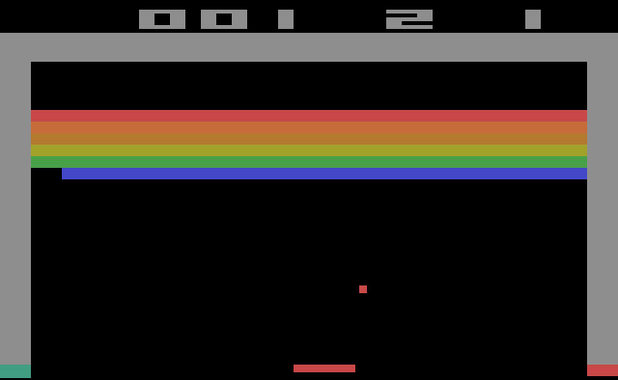
\includegraphics[width=0.99\linewidth]{figs/atari_breakout.jpg}
        \caption{Atari Breakout}
        \label{fig:breakout}
    \end{subfigure}%
    \begin{subfigure}{0.5\textwidth}
        
\includegraphics[width=0.99\linewidth]{figs/atari_breakout_bw.jpg}
        \caption{Black and white Breakout}
        \label{fig:bw_breakout}
    \end{subfigure}
    \caption{Atari Breakout. \ref{fig:breakout} is what Breakout looks like. We have the paddle in the bottom of the screen aiming to hit the ball in order to break the tiles at the top of the screen. \ref{fig:bw_breakout} is our transformation of Atari Breakout into black and white pixels for the purpose of some of the following problems.}
    \label{fig:my_label}
\end{figure}
% 

\begin{enumerate}
\item \textbf{[1 points]} Suppose we are dealing with the black and white version of Breakout\footnote{Play a Google-Doodle version \href{http://goo.gl/hb5xa}{here}} as in Figure~\ref{fig:bw_breakout}. Furthermore, suppose we are representing the state of the game as just a vector of pixel values without considering if a certain pixel is always black or white. Since we are dealing with the black and white version of the game, these pixel values can either be 0 or 1.

What is the size of the state space?

\begin{tcolorbox}[fit,height=1cm, width=\linewidth, blank, borderline={1pt}{-2pt},nobeforeafter]
%solution
Considering all the possible combinations of black and white pixels corresponding to the given resolution, the size of the state space is: $2^{160*192}=2^30720$
\end{tcolorbox}

    
\item \textbf{[1 points]} In the same setting as the previous part, suppose we wish to apply Q-learning to this problem. What is the size of the Q-value table we will need?

\begin{tcolorbox}[fit,height=1cm, width=\linewidth, blank, borderline={1pt}{-2pt},nobeforeafter]
%solution
$Q-table:\begin{bmatrix}size(state space) & x & actions \end{bmatrix}=\begin{bmatrix}2^{30720} & x & 3 \end{bmatrix}$
\end{tcolorbox}


\clearpage
\item \textbf{[1 points]} Now assume we are dealing with the colored version of Breakout as in Figure~\ref{fig:breakout}. Now each pixel is a tuple of real valued numbers between $0$ and $1$. For example, black is represented as $(0, 0, 0)$ and white is $(1, 1, 1)$. 

What is the size of the state space and Q-value table we will need?

\begin{tcolorbox}[fit,height=1cm, width=\linewidth, blank, borderline={1pt}{-2pt},nobeforeafter]
%solution
$Q-table:\begin{bmatrix}size(state space) & x & actions \end{bmatrix}=\begin{bmatrix}Infinity & x & 3 \end{bmatrix}$
\end{tcolorbox}
\end{enumerate}

By now you should see that we will need a huge table in order to apply Q-learning (and similarly value iteration and policy iteration) to Breakout given this state representation. This table would not even fit in the memory of any reasonable computer! Now this choice of state representation is particularly na\"ive. If we choose a better state representation, we could drastically reduce the table size needed. 

On the other hand, perhaps we don't want to spend our days feature engineering a state representation for Breakout. Instead we can apply function approximation to our reinforcement algorithms! The whole idea of function approximation is that states nearby to the state of interest should have \emph{similar} values. That is, we should be able to generalize the value of a state to nearby and unseen states.

Let us define $q_\pi(s, a)$ as the true action value function of the current policy $\pi$. Assume $q_\pi(s,a)$ is given to us by some oracle. Also define $q(s, a; \wv)$ as the action value predicted by the function approximator parameterized by $\wv$. Here $\wv$ is a matrix of size $|\mathcal{S}| \times |\mathcal{A}|$. Clearly we want to have $q(s, a; \wv)$ be close to $q_\pi(s, a)$ for all $(s, a)$ pairs we see. This is just our standard regression setting. That is, our objective function is just the Mean Squared Error:
\begin{align}
J(\wv) = \frac{1}{2} \frac{1}{N} \sum_{s\in\mathcal{S}, a\in\mathcal{A}} \left(q_\pi(s, a) - q(s, a; \wv) \right)^2
\end{align}
Because we want to update for each example stochastically\footnote{This isn't really stochastic, you'll be asked in a bit why.}, we get the following update rule:
\begin{align}
\wv \leftarrow \wv - \alpha \left(q(s, a; \wv) - q_\pi(s,a) \right) \nabla_\wv q(s, a; \wv)
\end{align}

However, more often then not\footnote{Always in real life.} we will not have access to the oracle that gives us our target $q_\pi(s, a)$. So how do we get the target to regress $q(s, a; \wv)$ on? One way is to bootstrap\footnote{Metaphorically, the agent is pulling itself up by its own bootstraps.} an estimate of the action value under a greedy policy using the function approximator itself. That is to say
\begin{align}
q_\pi (s, a) \approx r + \gamma \max_{a'} q(s', a'; \wv)
\end{align}
Where $r$ is the reward observed from taking action $a$ at state $s$, $\gamma$ is the discount factor and $s'$ is the state resulting from taking action $a$ at state $s$. This target is often called the Temporal Difference (TD) target, and gives rise to the following update for the parameters of our function approximator in lieu of a tabular update:

\begin{align}
\wv \leftarrow \wv - \alpha \bigg( \underbrace{q(s, a; \wv) - \underbrace{\big (r + \gamma \max_{a'}q(s', a'; \wv)\big)}_{\text{TD Target}}}_{\text{TD Error}} \bigg) \nabla_\wv q(s, a; \wv)
\end{align}

\begin{enumerate}
\setcounter{enumi}{3}
\item \textbf{[2 points]} Let us consider the setting where we can represent our state by some vector $\sv$, action $a \in \{0, 1, 2\}$ and we choose a linear approximator. That is:
\begin{align}
\label{eq:linearEQ}
q(\sv, a; \wv) = \sv^T\wv_a
\end{align}
Again, assume we are in the black and white setting of Breakout as in Figure~\ref{fig:bw_breakout}. Show that tabular Q-learning is just a special case of Q-learning with a linear function approximator by describing a construction of $\sv$. (\textbf{Hint}: Engineer features such that \ref{eq:linearEQ} encodes a table lookup)

\begin{tcolorbox}[fit,height=4cm, width=\linewidth, blank, borderline={1pt}{-2pt},nobeforeafter]
%solution
\end{tcolorbox}


\item \textbf{[3 points]} Stochastic Gradient Descent works because we can assume that the samples we receive are independent and identically distributed. Is that the case here? If not, why and what are some ways you think you could combat this issue?

\begin{tcolorbox}[fit,height=3cm, width=\linewidth, blank, borderline={1pt}{-2pt},nobeforeafter]
%solution
\end{tcolorbox}


\end{enumerate}




\clearpage
\subsection{Empirical Questions \points{6}}

The following questions should be completed after you work through the programming portion of this assignment (Section \ref{sec:code}). 

\begin{enumerate}
\item \textbf{[4 points]} Run Q-learning on the mountain car environment using both tile and raw features. 

For the raw features: run for 2000 episodes with max iterations of 200, $\epsilon$ set to 0.05, $\gamma$ set to 0.999, and a learning rate of 0.001. 

For the tile features: run for 400 episodes with max iterations of 200, $\epsilon$ set to 0.05, $\gamma$ set to 0.99, and a learning rate of 0.00005.

For each set of features, plot the return (sum of all rewards in an episode) per episode on a line graph. On the same graph, also plot the rolling mean over a 25 episode window. Comment on the difference between the plots.

\begin{tcolorbox}[fit,height=12cm, width=\linewidth, blank, borderline={1pt}{-2pt},nobeforeafter]
%solution
\end{tcolorbox}

\end{enumerate}


\begin{figure}[H]
    \centering
    \begin{subfigure}{0.5\textwidth}
        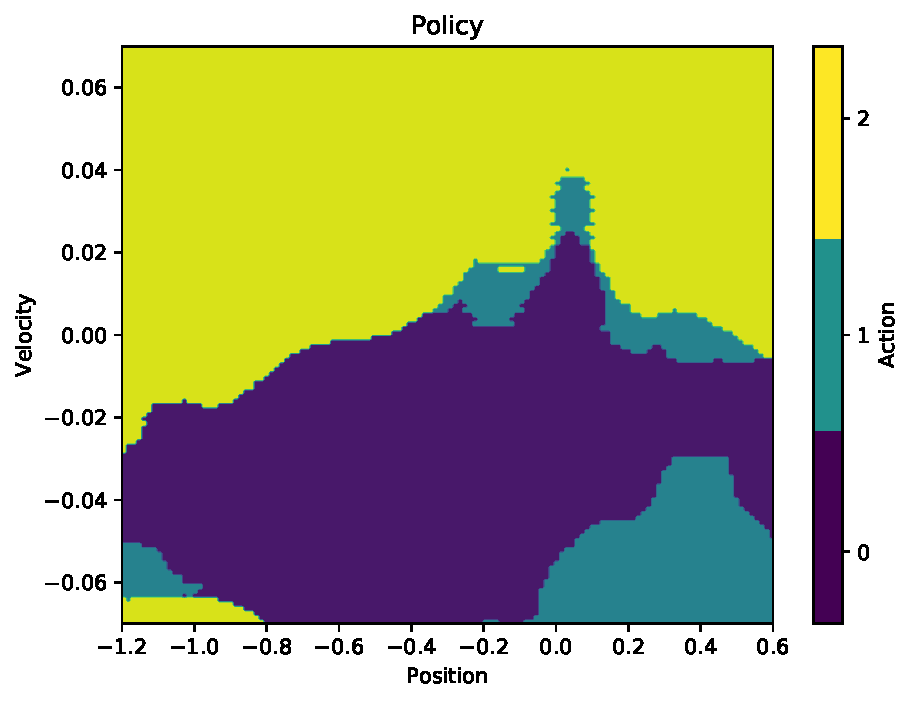
\includegraphics[width=\linewidth]{figs/policy_A.pdf}
        \caption{}
        \label{fig:policy_a}
    \end{subfigure}%
    \begin{subfigure}{0.5\textwidth}
        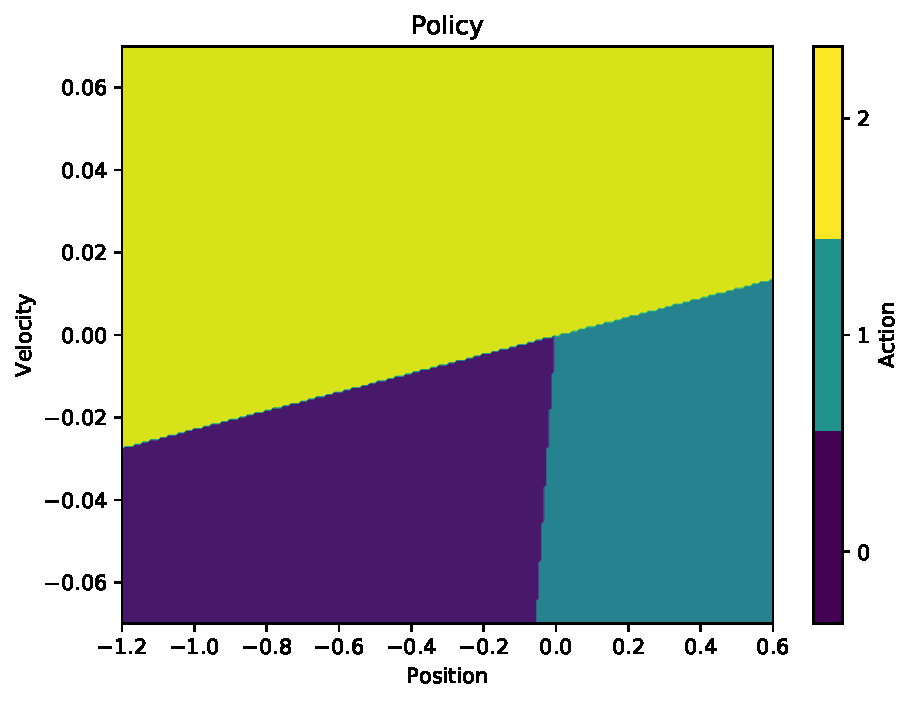
\includegraphics[width=\linewidth]{figs/policy_B.pdf}
        \caption{}
        \label{fig:policy_b}
    \end{subfigure}
    \caption{Estimated optimal policy visualizations for both types of features}
    \label{fig:policy}
\end{figure}


\begin{enumerate}
\setcounter{enumi}{1}
\item \textbf{[2 points]} We have created visualizations of the potential policies learned. For each plot in Figure~\ref{fig:policy} write down which features (raw or tile) were likely used in Q-learning with function approximation. Explain your reasoning. In addition, interpret each of these plots in the context of the mountain car environment.
    
\begin{tcolorbox}[fit,height=4cm, width=\linewidth, blank, borderline={1pt}{-2pt},nobeforeafter]
%solution
\end{tcolorbox}

\end{enumerate}


% Ideas: 
% Introduce the environment, discretization, and tiling (coarse coding)

\clearpage
\textbf{Collaboration Questions} Please answer the following:


    After you have completed all other components of this assignment, report your answers to the collaboration policy questions detailed in the Academic Integrity Policies found \href{http://www.cs.cmu.edu/~mgormley/courses/10601/about.html#7-academic-integrity-policies}{here}.
    \begin{enumerate}
        \item Did you receive any help whatsoever from anyone in solving this assignment? Is so, include full details.
        \item Did you give any help whatsoever to anyone in solving this assignment? Is so, include full details.
        \item Did you find or come across code that implements any part of this assignment ? If so, include full details.
    \end{enumerate}
    
\begin{tcolorbox}[fit,height=14cm, width=\linewidth, blank, borderline={1pt}{-2pt},nobeforeafter]
    %solution
     
\end{tcolorbox}


\clearpage
\section{Programming \points{60}}
\label{sec:code}

Your goal in this assignment is to implement Q-learning with linear function approximation to solve the mountain car environment. You will implement all of the functions needed to initialize, train, evaluate, and obtain the optimal policies and action values with Q-learning. In this assignment we will provide the environment for you.

The program you write will be automatically graded using the Autolab system. You may write your program in \textbf{Octave/MATLAB, Python, Java, or C++}. However, you should use the same language for all parts below. For this assignment, we heavily suggest \textbf{not} to use octave/MATLAB.

\textbf{Octave/MATLAB users}: Note that we will be manually grading your code using MATLAB for this assignment only. This means that the autograder will not grade your code on submission. This is because Octave's \texttt{collections.Map} is too slow for the assignment's purposes. We heavily suggest you use one of the other three languages instead, since our reference solution takes 400 seconds on MATLAB and much longer on octave.

\subsection{Specification of Mountain Car}
In this assignment, you will be given code that fully defines the Mountain Car environment. In Mountain Car you control a car that starts at the bottom of a valley. Your goal is to reach the flag at the top right, as seen in Figure~\ref{fig:mountaincar}. However, your car is under-powered and can not climb up the hill by itself. Instead you must learn to leverage gravity and momentum to make your way to the flag. It would also be good to get to this flag as fast as possible.

\begin{figure}[H]
    \centering
    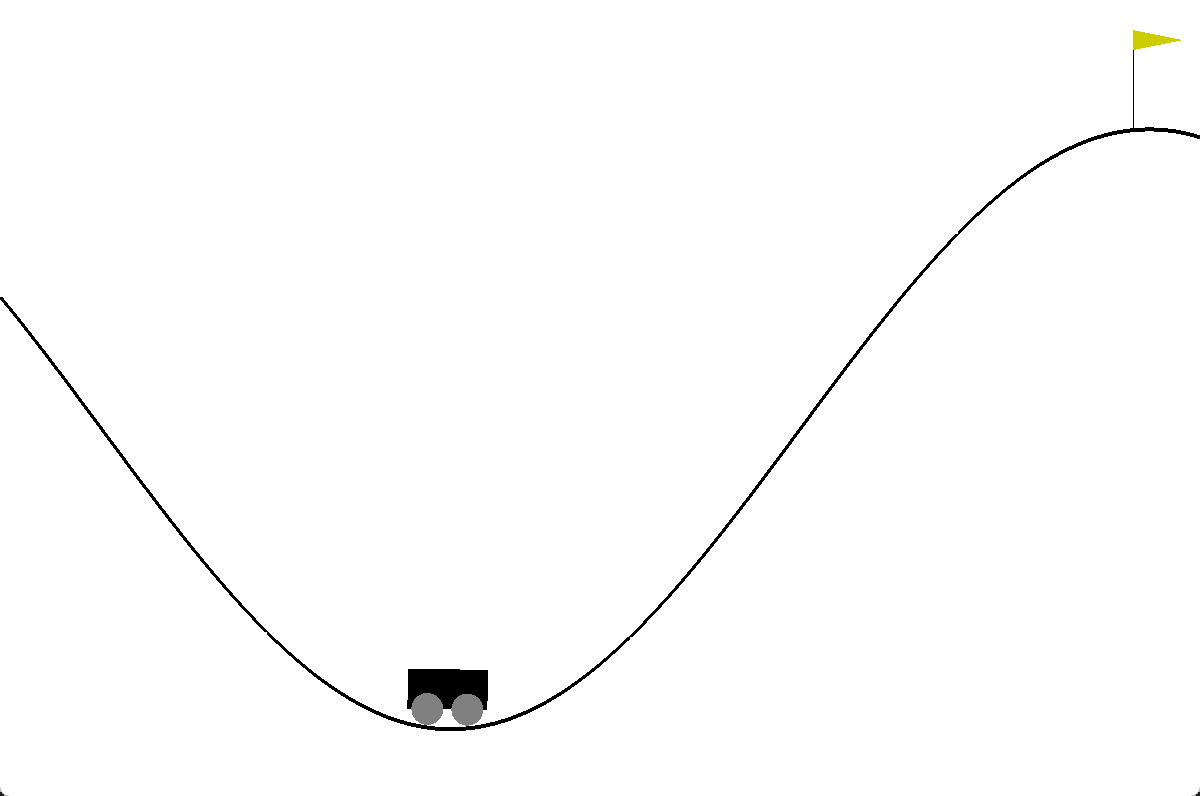
\includegraphics[width=0.5\linewidth]{figs/MountainCar.png}
    \caption{What the Mountain Car environment looks like. The car starts at some point in the valley. The goal is to get to the top right flag.}
    \label{fig:mountaincar}
\end{figure}

The state of the environment is represented by two variables, \texttt{position} and \texttt{velocity}. \texttt{position} can be between $-1.2$ and $0.6$ inclusive and \texttt{velocity} can be between $-0.07$ and $0.07$ inclusive. These are just measurements along the $x$-axis.

The actions that you may take at any state are $\{0, 1, 2\}$ which respectively correspond to (0) pushing the car left, (1) doing nothing, and (2) pushing the car right.

\subsection{Q-learning With Linear Approximations}
The Q-learning algorithm is a model-free reinforcement learning algorithm where we assume we don't have access to the model of the environment we're interacting with. We also don't build a complete model of the environment during the learning process. A learning agent interacts with the environment solely based on calls to \textbf{step} and \textbf{reset} methods of the environment. Then the Q-learning algorithm updates the q-values based on the values returned by these methods. Analogously, in the approximation setting the algorithm will instead update the parameters of q-value approximator.


Let the learning rate be $\alpha$ and discount factor be $\gamma$. Recall that we have the information after one interaction with the environment, $(s, a, r, s')$. The tabular update rule based on this information is: 
\[
    Q(s,a) = (1 - \alpha) Q(s, a) + \alpha \left(r + \gamma \max_{a'} Q(s', a')\right)
\]

Instead, for the function approximation setting we get the following update rule derived from Section~\ref{sec:FA}\footnote{Note that we have made the bias term explicit here, where before it was implicitly folded into $\wv$ }:

\[
\wv \leftarrow \wv - \alpha \left(q(\sv, a; \wv) - (r + \gamma \max_{a'} q(\sv', a'; \wv)\right) \nabla_\wv q(\sv, a; \wv)
\]

Where:

\[
q(\sv,a;\wv) = \sv^T \wv_a + b
\]

The epsilon-greedy action selection method selects the optimal action with probability $1 - \epsilon$ and selects uniformly at random from one of the 3 actions (0, 1, 2) with probability $\epsilon$. The reason that we use an epsilon-greedy action selection is we would like the agent to do explorations as well. For the purpose of testing, we will test two cases: $\epsilon = 0$ and $0 < \epsilon < 1$. When $\epsilon = 0$, the program becomes deterministic and your output have to match our reference output accurately. In this case, if there is a draw in the greedy action selection process, pick the action represented by the smallest number. For example, if we're at state $s$ and $Q(s, 0) = Q(s, 2)$, then take action $0$. And when $0 < \epsilon < 1$, your reference output will need to fall in a certain range that we determine by running exhaustive experiments based on the input parameters.


\subsection{Feature Engineering}
Linear approximations are great in their ease of use and implementations. However, there sometimes is a downside; they're \emph{linear}. This can pose a problem when we think the value function itself is nonlinear with respect to the state. For example, we may want the value function to be symmetric about 0 velocity. To combat this issue we could throw a more complex approximator at this problem, like a neural network. But we want to maintain simplicity in this assignment, so instead we will look at a nonlinear transformation of the ``raw'' state.

\begin{figure}[H]
\centering
\begin{subfigure}{0.5\textwidth}

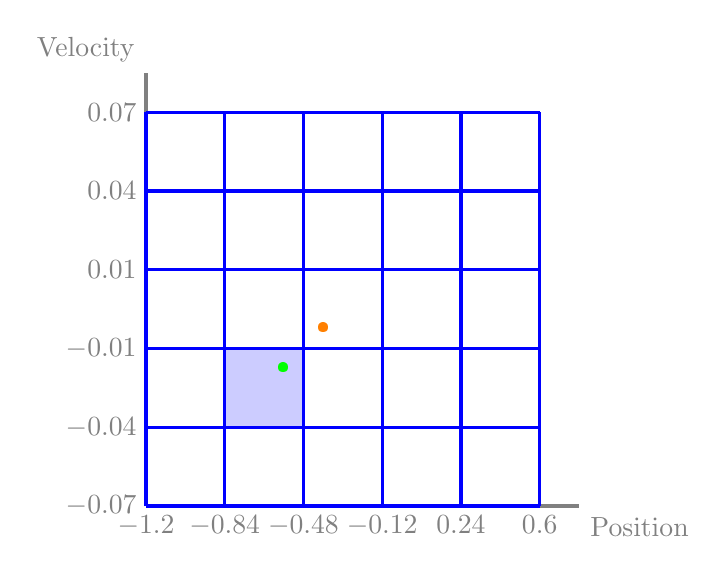
\begin{tikzpicture}[scale=1.0]
\pgfkeys{/pgf/number format/.cd,fixed,precision=2}
% Draw labels
\draw [ultra thick,gray,] (0,0)--(5.5,0) node[below right] {\text{Position}};
\draw [ultra thick,gray,] (0,0)--(0,5.5) node[above left] {\text{Velocity}};
% Draw axis
\newcommand*{\xMin}{0}%
\newcommand*{\xMax}{5}%
\newcommand*{\yMin}{0}%
\newcommand*{\yMax}{5}%
    \foreach \i in {\xMin,...,\xMax} {
        \draw [very thin,gray] (\i,\yMin) -- (\i,\yMax)  node [below] at (\i,\yMin) {\pgfmathparse{(\i/50)*18-1.2}$\pgfmathprintnumber{\pgfmathresult}$};
    }
    \foreach \i in {\yMin,...,\yMax} {
        \draw [very thin,gray] (\xMin,\i) -- (\xMax,\i) node [left] at (\xMin,\i) {\pgfmathparse{(\i/500)*14-0.07}$\pgfmathprintnumber{\pgfmathresult}$};
    }
% Draw grids
\draw [step=1.0,blue, very thick] (0.0,0.0) grid (5.0,5.0);
% \draw [very thick, red, step=1.0cm,xshift=-0.5cm, yshift=-0.5cm] (0.5,0.5) grid +(5.0,5.0);

% Draw shaded regions
\fill [blue, opacity=0.2] (1,1) rectangle (2,2);
% \fill [red, opacity=0.2] (1.5,1.5) rectangle (2.5,2.5);

% Draw point
\node [green] at (1.75,1.75) {\textbullet};
\node [orange] at (2.25, 2.25) {\textbullet};

\end{tikzpicture}
\caption{A discretization of the state space of Mountain Car}
\label{fig:discrete}
\end{subfigure}%
\begin{subfigure}{0.5\textwidth}

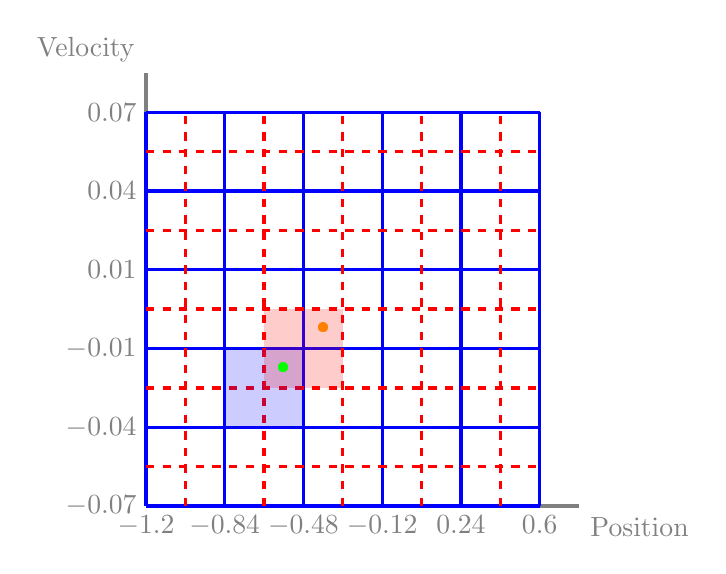
\begin{tikzpicture}[scale=1.0]
\pgfkeys{/pgf/number format/.cd,fixed,precision=2}
% Draw labels
\draw [ultra thick,gray,] (0,0)--(5.5,0) node[below right] {\text{Position}};
\draw [ultra thick,gray,] (0,0)--(0,5.5) node[above left] {\text{Velocity}};
% Draw axis
\newcommand*{\xMin}{0}%
\newcommand*{\xMax}{5}%
\newcommand*{\yMin}{0}%
\newcommand*{\yMax}{5}%
    \foreach \i in {\xMin,...,\xMax} {
        \draw [very thin,gray] (\i,\yMin) -- (\i,\yMax)  node [below] at (\i,\yMin) {\pgfmathparse{(\i/50)*18-1.2}$\pgfmathprintnumber{\pgfmathresult}$};
    }
    \foreach \i in {\yMin,...,\yMax} {
        \draw [very thin,gray] (\xMin,\i) -- (\xMax,\i) node [left] at (\xMin,\i) {\pgfmathparse{(\i/500)*14-0.07}$\pgfmathprintnumber{\pgfmathresult}$};
    }
% Draw grids
\draw [step=1.0,blue, very thick] (0.0,0.0) grid (5.0,5.0);
\draw [very thick, dashed, red, step=1.0cm,xshift=-0.5cm, yshift=-0.5cm] (0.5,0.5) grid +(5.0,5.0);

% Draw shaded regions
\fill [blue, opacity=0.2] (1,1) rectangle (2,2);
\fill [red, opacity=0.2] (1.5,1.5) rectangle (2.5,2.5);

% Draw point
\node [green] at (1.75,1.75) {\textbullet};
\node [orange] at (2.25, 2.25) {\textbullet};

\end{tikzpicture}
\caption{A tiling of the state space of Mountain Car}
\label{fig:tiling}
\end{subfigure}

\caption{State representations for the states of Mountain Car}
\label{fig:states}
\end{figure}

For the Mountain Car environment, we know that \texttt{position} and \texttt{velocity} are both bounded. What we can do is draw a grid over the possible \texttt{position}-\texttt{velocity} combinations as seen in Figure~\ref{fig:discrete}. We then enumerate the grid from bottom left to top right, row by row. Then we map all states that fall into a grid square with the corresponding one-hot encoding of the grid number. For efficiency reasons we will just use the index that is non-zero. For example the green point would be mapped to $\{6\}$. This is called a \emph{discretization} of the state space.

The downside to the above approach is that although observing the green point will let us learn parameters that generalize to other points in the shaded blue region, we will not be able to generalize to the orange point even though it is nearby. We can instead draw two grids over the state space, each offset slightly from each other as in Figure~\ref{fig:tiling}. Now we can map the green point to two indices, one for each grid, and get $\{6, 39\}$. Now the green point has parameters that generalize to points that map to $\{6\}$ (the blue shaded region) in the first discretization and parameters that generalize to points that map to $\{39\}$ (the red shaded region) in the second. We can generalize this to multiple grids, which is what we do in practice. This is called a \emph{tiling} or a \emph{coarse-coding} of the state space. 


\subsection{Implementation Details}
Here we describe the API to interact with the Mountain Car environment available to you in Python. The other languages will have an analagous API.

\begin{itemize}
    \item \texttt{\_\_init\_\_(mode)}: Initializes the environment to the a mode specified by the value of \texttt{mode}. This can be a string of either ``raw'' or ``tile''. 
    
    ``raw'' mode tells the environment to give you the state representation of raw features encoded in a sparse format: $\{0 \rightarrow \texttt{position}, 1 \rightarrow \texttt{velocity}\}$.
    
    In ``tile'' mode you are given indices of the tiles which are active in a sparse format: $\{T_1 \rightarrow 1, T_2 \rightarrow 1, \ldots T_n \rightarrow 1\}$ where $T_i$ is the tile index for the $i$th tiling. All other tile indices are assumed to map to 0. For example the state representation of the example in Figure~\ref{fig:tiling} would become $\{6 \rightarrow 1, 39 \rightarrow 1\}$.
    
    The size of the state space of the ``raw'' mode is 2. The size of the state space of the ``tile'' mode is 2048. These values can be accessed from the environment through the \texttt{state\_space} property, and similarly for other languages.
    \item \texttt{reset()}: Reset the environment to starting conditions.
    \item \texttt{step(action)}: Take a step in the environment with the given action. \texttt{action} must be either $0$, $1$ or $2$. This will return a tuple of $(\texttt{state}, \texttt{reward}, \texttt{done})$ which is the next state, the reward observed, and a boolean indicating if you reached the goal or not, ending the episode. The \texttt{state} will be either a raw' or tile representation, as defined above, depending on how you initialized Mountain Car.  If you observe \texttt{done = True} then you should \texttt{reset} the environment and end the episode. Failure to do so will result in undefined behavior.
    \item \textbf{[Python Only]} \texttt{render(self)}: Optionally render the environment. It is computationally intensive to render graphics, so only render a full episode once every 100 or 1000 episodes. Requires the installation of \texttt{pyglet}. This will be a no-op in autolab.
\end{itemize}

You should now implement your Q-learning algorithm with linear approximations as \newline\texttt{q\_learning.\{py|java|cpp|m\}}. The program will assume access to a given environment file(s) which contains the Mountain Car environment which we have given you. Initialize the parameters of the linear model with all 0 (and don't forget to include a bias!) and use the epsilon-greedy strategy for action selection.

Your program should write a output file containing the total rewards (the returns) for every episode after running Q-learning algorithm. There should be one return per line.

Your program should also write an output file containing the weights of the linear model. The first line should be the value of the bias. Then the following $|\mathcal{S}| \times |\mathcal{A}|$ lines should be the values of weights, outputted in row major order\footnote{\url{https://en.wikipedia.org/wiki/Row-_and_column-major_order}}, assuming your weights are stored in a $|\mathcal{S}| \times |\mathcal{A}|$ matrix.

The autograder will use the following commands to call your function:

\begin{tabbing}
For Python: \=\texttt{\$ \textbf{python} q\_learning.\textbf{py} [args\dots]}\\
For Java: \>\texttt{\$ \textbf{javac} -cp "./lib/ejml-v0.33-libs/*:./" q\_learning.\textbf{java}};\\ \>  \texttt{\textbf{java} -cp "./lib/ejml-v0.33-libs/*:./" q\_learning [args\dots]}\\
For C++: \>\texttt{\$ \textbf{g++} -g -std=c++11 -I./lib q\_learning.\textbf{cpp}; ./a.out [args\dots]}\\
% For Octave: \>\texttt{\$ \textbf{octave} -qH q\_learning.\textbf{m} [args\dots]}
\end{tabbing}

Where above \texttt{[args\dots]} is a placeholder for command-line arguments: \texttt{<mode>} \texttt{<weight\_out>} \texttt{<returns\_out>} \texttt{<episodes>} \texttt{<max\_iterations>} \texttt{<epsilon>} \texttt{<gamma>} \texttt{<learning\_rate>}. These arguments are described in detail below:
\begin{enumerate}
    \item \texttt{<mode>}: mode to run the environment in. Should be either \texttt{``raw''} or \texttt{``tile''}.
    \item \texttt{<weight\_out>}: path to output the weights of the linear model.
    \item \texttt{<returns\_out>}: path to output the returns of the agent
    \item \texttt{<episodes>}: the number of episodes your program should train the agent for. One episode is a sequence of states, actions and rewards, which ends with terminal state or ends when the maximum episode length has been reached.
    \item \texttt{<max\_iterations>}: the maximum of the length of an episode. When this is reached, we terminate the current episode.
    \item \texttt{<epsilon>}: the value $\epsilon$ for the epsilon-greedy strategy
    \item \texttt{<gamma>}: the discount factor $\gamma$.
    \item \texttt{<learning\_rate>}: the learning rate $\alpha$ of the Q-learning algorithm
\end{enumerate}


Example command for python users:
\begin{lstlisting}[language=Shell]
$ python q_learning.py raw weight.out returns.out \ 
 4 200 0.05 0.99 0.01
\end{lstlisting}

Example output from running the above command (your code won't match exactly, but should be close).

\texttt{<weight\_out>}
\begin{lstlisting}
-7.6610506220312296
1.3440159024460183
1.344872959883069
1.340055578403996
-0.0007770480987990149
0.0011306483117300896
0.0017559989206646666
\end{lstlisting}

\texttt{<returns\_out>}
\begin{lstlisting}
-200.0
-200.0
-200.0
-200.0
\end{lstlisting}

\subsection{Autolab Submission}
You must submit a .tar file 
named \texttt{rl.tar} containing \texttt{q\_learning.\{py|m|java|cpp\}}.  

You can create that file by running:
\begin{lstlisting}
tar -cvf rl.tar q_learning.{py|m|java|cpp}
\end{lstlisting}
from the directory containing your code. You may make up to \textbf{10 submissions} to Autolab before the deadline, but only your last submission will be graded.

Some additional tips: {\bf DO NOT} compress your files; you are just
creating a tarball. Do not use tar \texttt{-czvf}.  {\bf DO NOT} put
the above files in a folder and then tar the folder.  Autolab is case
sensitive, so observe that all your files should be named in {\bf
  lowercase}. You must submit this file to the corresponding homework
link on Autolab. The autograder for Autolab prints out some additional 
information about the tests that it ran. You can view this output by selecting 
 "Handin History" from the menu and then clicking one of the scores you 
 received for a submission. For example on this assignment, among other things, 
 the autograder will print out which language it detects (e.g. Python, Octave, C++, Java). 
 
 \begin{notebox}
  {\bf Python3 Users:} Please include a blank file called python3.txt (case-sensitive) in your tar submission and we will execute your submitted program using Python 3 instead of Python 2.7. Please do not rely on any ordering of dictionary elements.
 \end{notebox}

%\clearpage

\begin{notebox}
\paragraph{Linear Algebra Libraries} It is often more convenient to have a linear algebra library at your disposal. In this assignment, Java users may use EJML\footnote{\url{https://ejml.org}} and C++ users Eigen\footnote{\url{http://eigen.tuxfamily.org/}}. Details below. 
%
(As usual, Python users have numpy; Octave users have built-in matrix support.)
%
\begin{description}
\item[Java] EJML is a pure Java linear algebra package with three interfaces. We strongly recommend using the SimpleMatrix interface. Autolab will use EJML version 3.3. The command line arguments above demonstrate how we will call you code. The classpath inclusion \lstinline{-cp "./lib/ejml-v0.33-libs/*:./"} will ensure that all the EJML jars are on the classpath as well as your code. 
\item[C++] Eigen is a header-only library, so there is no linking to worry about---just \lstinline{#include} whatever components you need. Autolab will use Eigen version 3.3.4. The command line arguments above demonstrate how we will call you code. The argument \lstinline{-I./lib} will include the \lstinline{lib/Eigen} subdirectory, which contains all the headers.
\end{description} 
We have included the correct versions of EJML/Eigen in the handout.tar for your convenience. Do {\bf not} include EJML or Eigen in your Autolab submission tar; the autograder will ensure that they are in place. 
\end{notebox}
%\appendix
%\input{appendix}

%\bibliographystyle{abbrv}
%\bibliography{bibliography}


\end{document}

